\section{数据校验}
% --- 工具 ---------------------------------------------------------------------
\subsection{下载工具}
\begin{frame}
    从gitee下载最新版的订单检查工具,以1.0.0版本为例

    {\small\url{https://gitee.com/zhengxueke/check-laads-order/releases}}

    \begin{annotationimage}{width=\linewidth}{images/3.1下载工具.jpg}
        \draw[red,very thick](0.3,0.16) rectangle (0.56,0.2);
    \end{annotationimage}
\end{frame}
\begin{frame}
    \frametitle{解压文件}
    下载好的压缩包,一定要全部解压缩到本地文件夹后再操作。\\
    解压后如图
    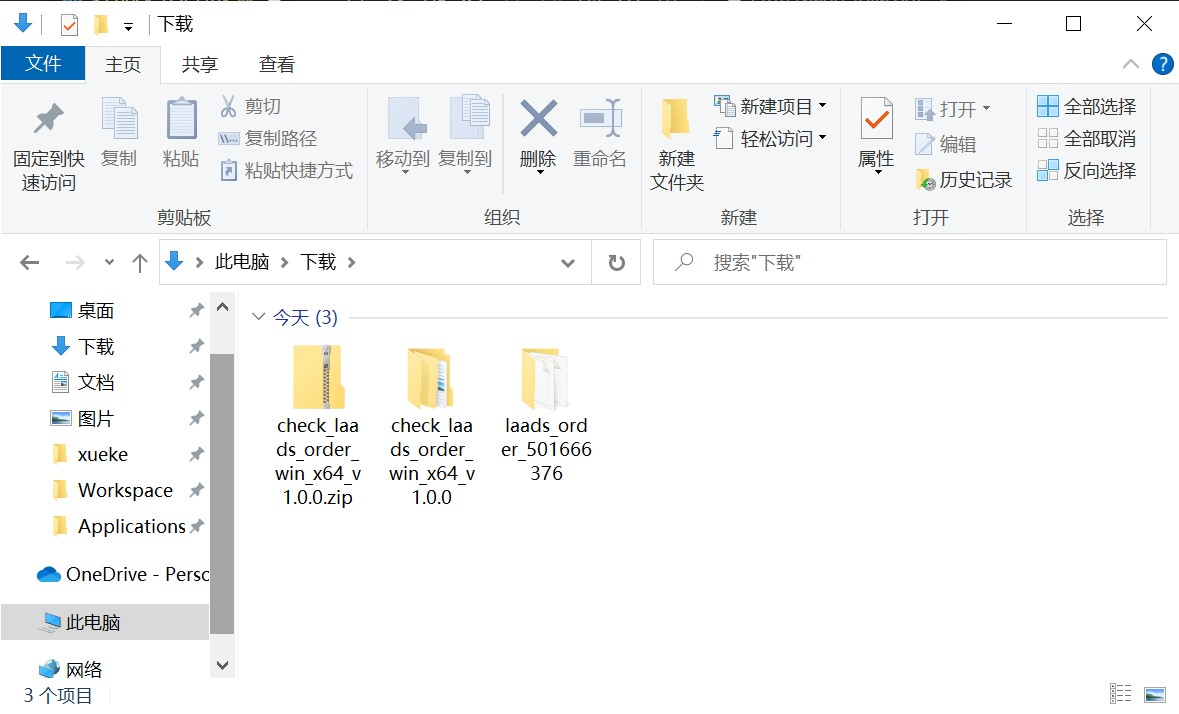
\includegraphics[width=\linewidth]{images/3.2解压}
\end{frame}
% --- 检校 ---------------------------------------------------------------------
\subsection{执行校验}
\begin{frame}
    \frametitle{找到程序}
    打开check\_laads\_order.exe主应用程序
    \begin{figure}
        \begin{annotationimage}{width=0.8\linewidth}{images/3.3找到程序}
            \draw[red,very thick](0.22,0.24) rectangle (0.42,0.3);
        \end{annotationimage}
    \end{figure}
\end{frame}
\begin{frame}
    \frametitle{导入订单}
    点击导入订单按钮
    \begin{figure}
        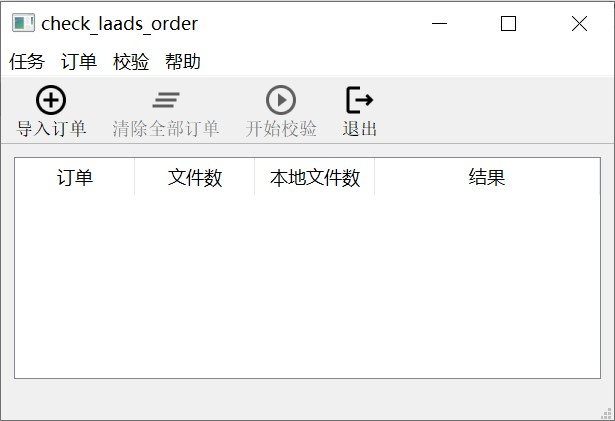
\includegraphics[width=0.8\linewidth]{images/3.4导入订单按钮}
    \end{figure}
\end{frame}
\begin{frame}
    \frametitle{选择订单文件夹}
    选择订单文件所在的文件夹,以我们在上文建立的文件夹为例
    \begin{figure}
        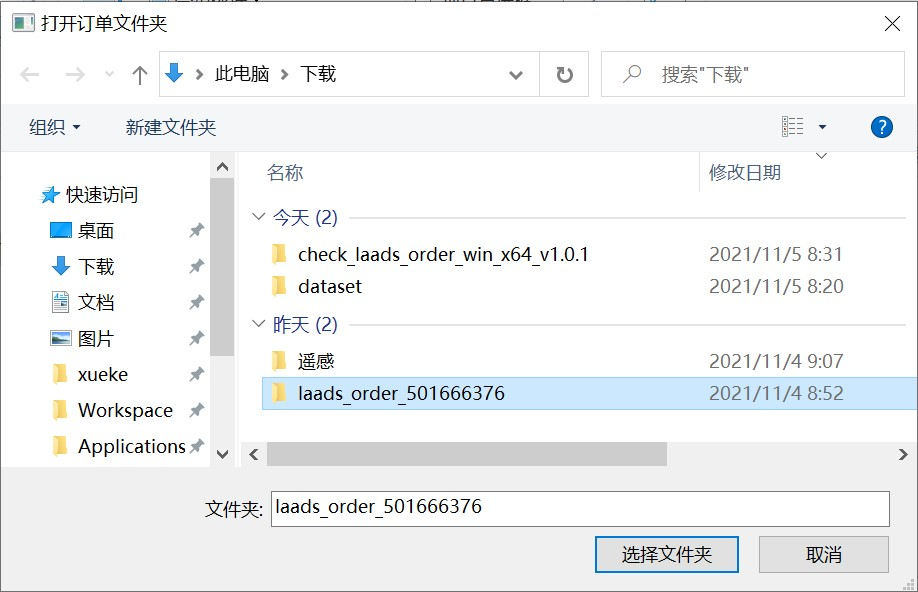
\includegraphics[width=0.8\linewidth]{images/3.5选择订单文件夹}
    \end{figure}
\end{frame}
\begin{frame}
    \frametitle{导入结果}
    软件会显示一些订单信息
    \begin{figure}
        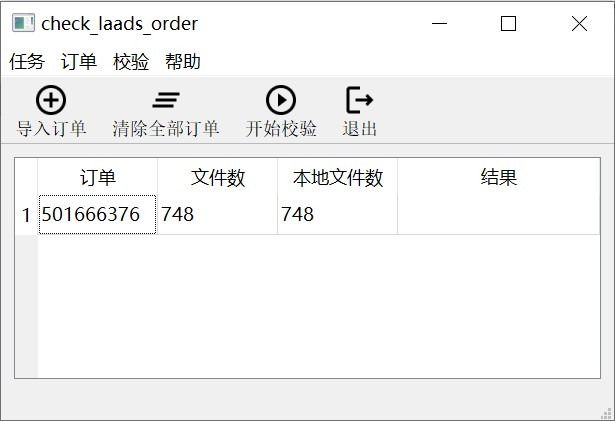
\includegraphics[width=0.8\linewidth]{images/3.6导入结果}
    \end{figure}
\end{frame}
\begin{frame}
    \frametitle{批量导入订单}
    本软件也可以批量导入订单。\\
    假如Dataset文件夹下有三个订单文件夹,我们想对这三个订单进行校验,
    那么我们只需要选择Dataset文件夹即可。
    \begin{figure}
        \begin{annotationimage}{width=0.6\linewidth}{images/3.9导入多个订单文件夹}
            \imagelabelset{annotation font = \normalfont\scriptsize}
            \draw[red,very thick](0.28,0.5) rectangle (0.74,0.66);
            \draw[annotation left = {三个订单 at 0.4}] to (0.3,0.52);
        \end{annotationimage}
    \end{figure}
\end{frame}
\begin{frame}
    \frametitle{批量导入效果}
    程序会识别每一个订单并显示信息
    \begin{figure}
        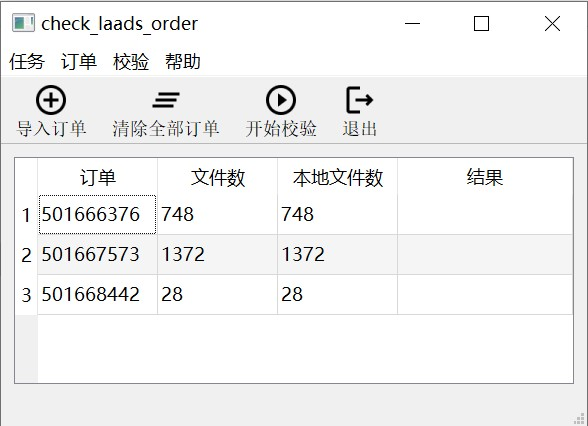
\includegraphics[width=0.8\linewidth]{images/3.10导入多个订单效果}
    \end{figure}
\end{frame}
\begin{frame}
    \frametitle{开始校验}
    点击\underline{开始校验}按钮,执行校验。
    \begin{figure}
        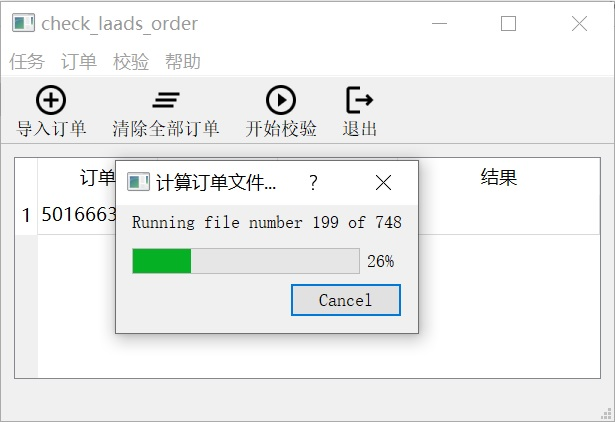
\includegraphics[width=0.8\linewidth]{images/3.7检查中}
    \end{figure}
\end{frame}
\begin{frame}
    \frametitle{校验结束}
    校验完成后,会在结果栏显示校验结果
    \begin{figure}
        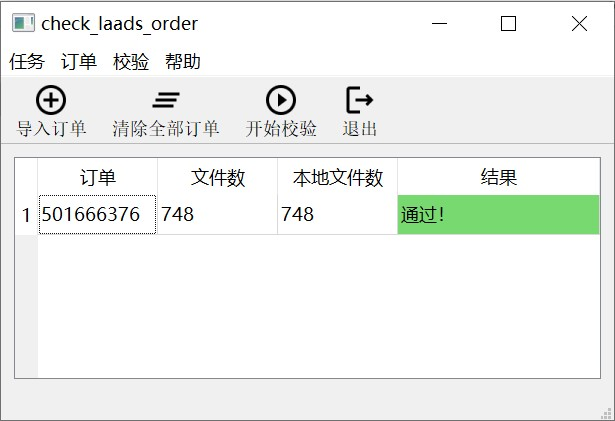
\includegraphics[width=0.8\linewidth]{images/3.8检查结果}
    \end{figure}
\end{frame}
% --- 结果 ---------------------------------------------------------------------
\subsection{如果订单有问题}
\frametitle{文件缺失或文件错误}
如果有错误,结果会标记为红色背景。
\begin{figure}
    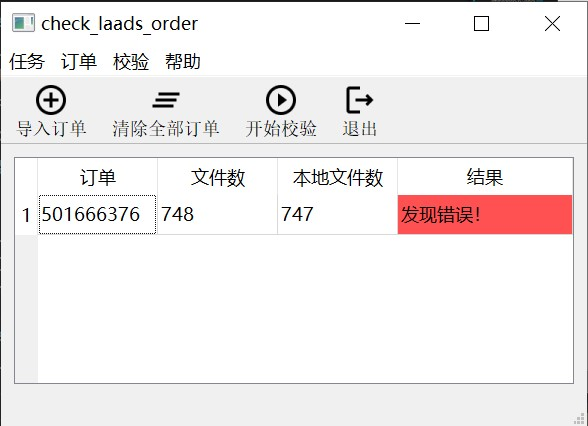
\includegraphics[width=0.8\linewidth]{images/3.11检查错误-文件缺失}
\end{figure}
\begin{frame}
    \frametitle{校验报告}
    双击红色单元格,可以打开检测报告
    \begin{figure}
        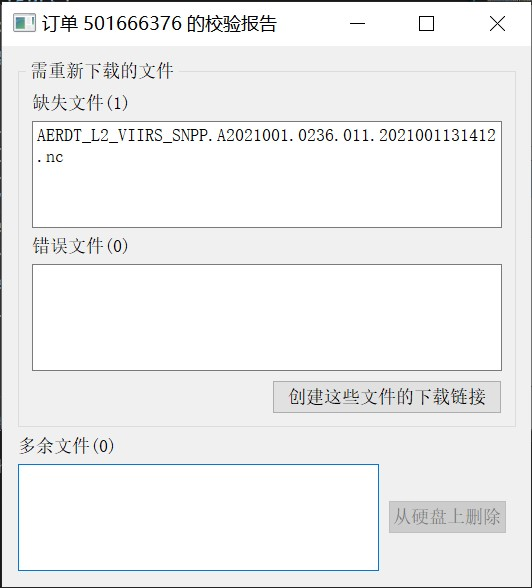
\includegraphics[width=0.5\linewidth]{images/3.12检测报告}
    \end{figure}
\end{frame}
\begin{frame}
    \frametitle{重新下载}
    如果想重新下载这些文件,可以点击创建下载链接按钮。\\
    \begin{figure}
        \begin{annotationimage}{width=0.5\linewidth}{images/3.12检测报告}
            \draw[red,very thick](0.5,0.28) rectangle (0.96,0.36);
        \end{annotationimage}
    \end{figure}
\end{frame}
\begin{frame}
    \frametitle{保存下载链接}
    默认会在订单文件夹内生成more\_download\_file\_links.txt文件
    点击保存即可
    \begin{figure}
        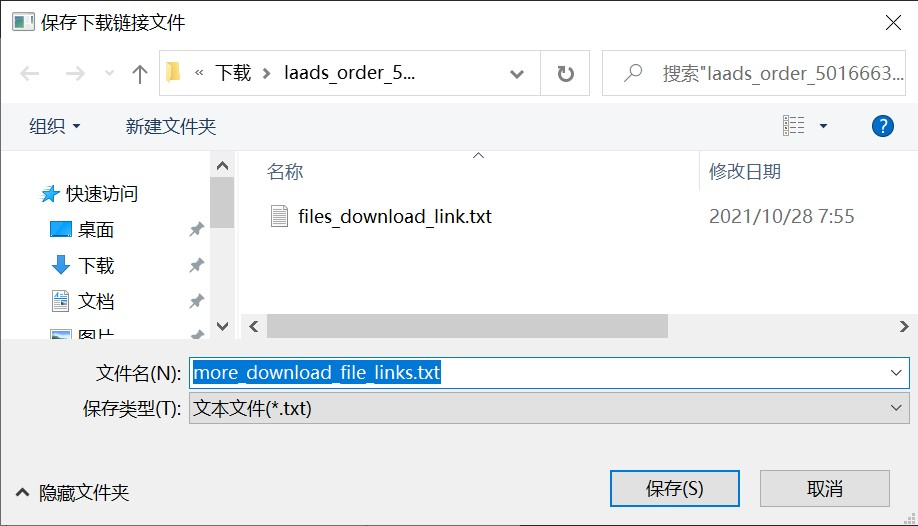
\includegraphics[width=0.8\linewidth]{images/3.13保存重新下载文件的链接}
    \end{figure}
\end{frame}

\begin{frame}
    \frametitle{重新下载}
使用与 \hyperlink{aria2-cmd}{\beamergotobutton{下载命令}} 类似方法,修改命令如下

aria2c.exe --http-use=登录laads的用户名 --http-passw=登录laadsd的密码
    --continue=true --retry-wait=2 -x 6 -i more\_download\_file\_links.txt
    --allow-overwrite

\begin{itemize}
    \item 替换成了我们的新生成的下载链接文件
    \item 加上了--allow-overwrite选项,允许覆盖本地已有文件
\end{itemize}
\end{frame}


